\documentclass{beamer}
\usepackage{youngtab}
\usepackage{verbatim}
\usepackage{graphicx}
\usepackage{subscaption}

\usetheme{boxes}
\usepackage{tikz}
\usetikzlibrary{decorations.pathmorphing}

\usecolortheme{seahorse}
\setbeamertemplate{footline}[frame number]

\usepackage{amsmath}
\usepackage{tikz}

% natural numbers
\def\nats{{\mathbb N}}

% Editorial
\newcommand*{\TODO}[1]{\textcolor{red}{TODO: #1}}
\newcommand*{\NOTE}[1]{\textcolor{blue}{Note: #1}}

\newcommand{\ind}[1]{\{1,\dots,#1\}}

\expandafter\def\expandafter\insertshorttitle\expandafter{%
  \insertshorttitle\hfill%
  \insertframenumber\,/\,\inserttotalframenumber}

\newcommand{\qtwid}{0.5\textwidth}
% Figure command. Might use later
\newcommand{\fig}[3]{
			\vspace{#2}
			\begin{center}
			Figure \thelecnum.#1:~#3
			\end{center}
	}
\title{Visualizing Integer Partitions}
\author[Salahub]{Chris Salahub}
\institute[UW]{University of Waterloo}

\begin{document}

\frame{\titlepage}

\frame{\frametitle{Presentation Outline}
We study congruence properties of the partition function. 
\begin{enumerate}
\item What are partitions? Objects from combinatorics, number theory, representation theory and physics.
\item Why do we care? \textbf{Generating functions, useful analytic identities, building blocks for counting discrete objects}.
\item How do we visualize them? \texttt{vispart}
\item Future work. 
\end{enumerate}
}
\frame{\frametitle{Integer Partitions}
Fix $n\in\nats_0$ an integer. We say that $\lambda = (\lambda_1,\lambda_2,\ldots,\lambda_k) \in \nats^k$ is a \emph{partition} of $n$ with $k\in\nats_0$ parts if 
$$\lambda_1\geq \lambda_2\geq \dotsb \geq\lambda_k$$
and
$$|\lambda|=\lambda_1+\lambda_2+\dotsb+\lambda_k = n.$$
We let $p(n)$ denote the total number of partitions of $n$, where we use the convention $p(0)=1$ and $p(n)=0$ for $n$ negative. 
}

\begin{frame}{The partitions of 4}
We note that $p(4) =5$ by enumerating the partitions of 4: 
\begin{align*}
4 &= 4\\
&= 3+1\\
&=2+2\\
&=2+1+1\\
&=1+1+1+1
\end{align*}
We see that there is only one partition with a single part: (4), two partitions with two parts: (3,1) and (2,2), one partition with three parts: (2,1,1), and a single partition with four parts: (1,1,1,1).

\end{frame}



\begin{frame} 
\frametitle{Ferrers Diagrams}
We can represents integer partitions geometrically using Ferrers diagrams,
\begin{center}
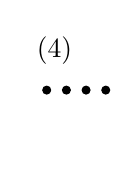
\begin{tikzpicture}
\draw (0.1,.5) node {$(4)$};
\foreach \x in {0,...,3}
	\filldraw (\x*.25, 0) circle (.5mm);
\foreach \x in {0,...,3}
	\filldraw[white] (\x*.25, -.25) circle (.5mm);\foreach \x in {0,...,3}
	\filldraw[white] (\x*.25, -.5) circle (.5mm);\foreach \x in {0,...,3}
	\filldraw[white] (\x*.25, -.75) circle (.5mm);
\end{tikzpicture}
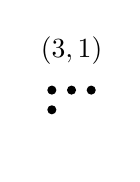
\begin{tikzpicture}
\draw (.5,.5) node {$(3,1)$};
\foreach \x in {0,...,2}
	\filldraw (0.25+\x*.25, 0) circle (.5mm);
\foreach \x in {0,...,0}
	\filldraw (0.25+\x*.25, -.25) circle (.5mm);\foreach \x in {0,...,3}
	\filldraw[white] (\x*.25, -.5) circle (.5mm);\foreach \x in {0,...,3}
	\filldraw[white] (\x*.25, -.75) circle (.5mm);\end{tikzpicture}
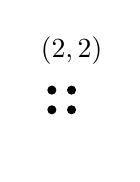
\begin{tikzpicture}
\draw (.5,.5) node {$(2,2)$};
\foreach \x in {0,...,1}
	\filldraw (0.25+\x*.25, 0) circle (.5mm);
\foreach \x in {0,...,1}
	\filldraw (0.25+\x*.25, -.25) circle (.5mm);\foreach \x in {0,...,3}
	\filldraw[white] (\x*.25, -.5) circle (.5mm);\foreach \x in {0,...,3}
	\filldraw[white] (\x*.25, -.75) circle (.5mm);\end{tikzpicture}
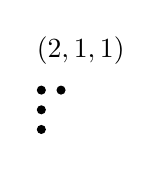
\begin{tikzpicture}
\draw (.5,.5) node {$(2,1,1)$};
\foreach \x in {0,...,1}
	\filldraw (\x*.25, 0) circle (.5mm);
\foreach \x in {0,...,0}
	\filldraw (\x*.25, -.25) circle (.5mm);\foreach \x in {0,...,0}
	\filldraw (\x*.25, -.5) circle (.5mm);\foreach \x in {0,...,3}
	\filldraw[white] (\x*.25, -.75) circle (.5mm);\end{tikzpicture}
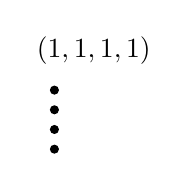
\begin{tikzpicture}
\draw (.5,.5) node {$(1,1,1,1)$};
\foreach \x in {0,...,0}
	\filldraw (\x*.25, 0) circle (.5mm);
\foreach \x in {0,...,0}
	\filldraw (\x*.25, -0.25) circle (.5mm);
\foreach \x in {0,...,0}
	\filldraw (\x*.25, -0.5) circle (.5mm);
\foreach \x in {0,...,0}
	\filldraw (\x*.25, -0.75) circle (.5mm);
\end{tikzpicture}
\end{center}
Or by using Young diagrams

$$\yng(4)\qquad \yng(3,1) \qquad \yng(2,2) \qquad \yng(2,1,1) \qquad \yng(1,1,1,1)$$

An alternative way of thinking of partitions is using an algebraic tool.
\end{frame}
\begin{frame}
\frametitle{Formal power series}
In general, we say that a sequence $(a_n)_{n\geq 0}$ has generating series $A(q)\in \nats[[q]]$ if $$A(q) = \sum_{n\geq 0}a_nq^n,$$
where the variable $x$ is variable only in the formal sense (usual algebraic properties hold, nothing analytic).

\end{frame}


\begin{frame}
\frametitle{Generating series for integer partitions}

If $P(q)$ is the generating series for integer partitions, then $P(q)$ has the closed form
$$P(q) = \sum_{n\geq0}p(n)q^n = \prod_{i\geq 1}\frac{1}{1-q^i}.$$


We can think of the right hand side as building blocks for each type of part in a partition. That is,
$$\frac{1}{1-q^i} = \sum_{j \geq 0}q^{ij} = 1 + q^i + q^{2i} +q^{3i} +\dotsb $$
represents the number of ways we could pick no parts of size $i$, the number of ways we could pick exactly one part of size $i$, exactly two parts of size $i$, three parts of size $i$,$\ldots$
\end{frame}

\begin{frame}
  \frametitle{Applications}
  The benefits of being able to visualize integer partitions are apparent when considering how many theorems can be proved using them.
\end{frame}

\begin{frame}
	\frametitle{Dufree squares}
\begin{theorem}
The generating series for integer partitions is equivalent to
$$P(q) = \prod_{i\geq 1} \frac{1}{1-q^i} = \sum_{k\geq1}x^{k^2}\prod_{i=1}^{k}\frac{1}{(1-q^i)^2}.$$	
\end{theorem}

\begin{proof}
\begin{center}
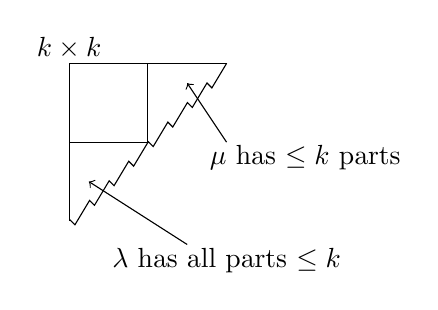
\begin{tikzpicture}
\draw (0,0) -- (1,0) -- (1,1) -- (0,1) -- (0,0);
\draw (1,1) -- (2,1);
\draw (0,0) -- (0,-1);
\draw[decorate, decoration=saw] (2,1) -- (0,-1);
\draw[->] (2,0) -- (1.5, .75);
\draw (3,-.2) node {$\mu$ has $\le k$ parts};
\draw[->] (1.5,-1.3) -- (.25, -.5);
\draw (2,-1.5) node {$\lambda$ has all parts $\le k$};
\draw (0,1.2) node {$k\times k$};

\end{tikzpicture}
\end{center}
\end{proof}
\end{frame}

 
\begin{frame}
	\frametitle{Self-conjugate partitions}
\begin{definition}
We say that a partition is self-conjugate partition if its reflection in $y = -x$ line is itself.	
\end{definition}

\begin{theorem}
The set of self-conjugate partitions is in bijection with the set of all partitions with distinct odd parts. In particular, if $s(n)$ is the number of self conjugate partitions of $n$, then
$$\sum_{n\geq 0}s(n)q^n = \prod_{i\geq 0}(1+q^{2i+1}).$$
\end{theorem}
\end{frame}  

\begin{frame}
\frametitle{Self-conjugate partitions}

\end{frame}

\begin{frame}
\frametitle{\texttt{vispart} }	
Our dependencies are 
\begin{itemize}
\item \texttt{partitions} - to list all partitions up to a particular value.
\item \texttt{grid} - in order to draw the partitions in a way that scales up.
\end{itemize}	

Our package allows one to 
\begin{itemize}
\item Draw any integer partition.
\begin{itemize}
\item Using either Ferrers diagrams or Young tableaux
\item Colour specific boxes; helps communicate specific properties of partitions.
\item Conjugation mapping is builtin.
\end{itemize}
\item Draw all integer partitions of $n$ for a fixed $n$.
\end{itemize}

\TODO{Demonstration with partitions of 4}

\end{frame}

\begin{frame}
\frametitle{Benefits of \texttt{vispart}}	
The benefits of \texttt{vispart} are as follows:

\begin{itemize}
	\item LaTeX's difficult to use for creating multiple partitions diagrams at once as LaTeX is generally not used for computation.
	\item To our knowledge, there is no implementation of the operation of conjugation within LaTeX.
	\item LaTeX's implementation of the partition diagrams does not do input handling.
	\item Maple, Matlab, Mathematica do not have built-in functionality for visualizing them to the best of our knowledge.
\end{itemize}
\end{frame}


\begin{frame}
\frametitle{Future work}	
In the study of symmetric functions, interest lies in assigning numbers within the boxes of a Young tableau.

\begin{itemize}
\item This helps communicate concepts from the theory of irreducible representations of the symmetric group $S_n$.
\item Provides an interpretation for \textbf{Littlewood-Richardson rule} which describes how to take a product of symmetric functions.
\end{itemize}

Improvements to the integer partition list generation.
\begin{itemize}
	\item Currently, \texttt{partitions} uses a recursive algorithm which relies on the recurrence:
	$$p(n,m) = \sum_{k=1}^{m}p(n-k, k).$$
	\item This algorithm is known to have $O(n\log n)$ time complexity and $O(n^2)$ space complexity.
\end{itemize}
\end{frame}

\end{document}
